% Provenance (never printed): see sources/outline_sources.md (Year 2: taphonomy; index fossils;
% facies and fossils as environment markers; reconstructing a palaeoenvironment from a map and a
% section). Taphonomy after Loron (2024); live, dead and fossil assemblages after Tyler and
% Kowalewski (2025); Lagerstaetten after Gaines and others (2024), Mussini and Butterfield
% (2025), Vannier and others (2018), Gerschermann and others (2021) and Rauhut and others
% (2018); zone durations after Al-Suwaidi and others (2022); ichnofacies after Buatois and others
% (2020) and Paz and others (2023); stenohaline groups after McGairy and others (2021) and Saleh
% and others (2022). The Varden column from figdata/shared/region.py; porosities and rates from
% figdata/bachelor-2/palaeoenv.py; exercise and problem values in the Book 4 scratch calculator
% calc/ch20.py. The fossil content given to the Varden units is invented, like the region.
\chapter{Fosil dan Paleolingkungan}\label{ch:b2:palaeoenvironments}

Pada sebongkah batu pasir kelabu terdapat tiga petunjuk: jejak yang dibajak seekor trilobit melalui lumpur,
riak yang ditinggalkan oleh arus, dan liang yang digali lalu ditinggalkan oleh seekor cacing. Tidak satu pun dari ketiganya adalah
hewan yang utuh, namun bersama-sama ketiganya menyatakan bahwa lereng bukit ini dulu adalah dasar laut, cukup dangkal
untuk diaduk oleh gelombang, dan cukup asin untuk dihuni trilobit. Fosil adalah
sisa dan jejak kehidupan masa lampau, dan ahli geologi membacanya dua kali: sebagai jam yang menentukan umur batuan,
dan sebagai saksi tempat batuan itu terbentuk. Bab ini mengikuti suatu makhluk hidup dari kematiannya
sampai ke laci kolektor, membuka endapan langka tempat bahkan tubuh lunak pun terawetkan, lalu membaca
lingkungan sebuah laut yang telah lenyap, dengan angka, dalam penutup sedimen Perbukitan Varden.
% ledger: usgs:fossil-record-bulk, loron24:taphonomy

\begin{recall}
\textbf{Dari volume-volume sekolah}: fosil, cetakan, tuangan, dan \omterm{def:b2:palaeoenvironments:fossil-kinds}{fosil jejak}; bagaimana penimbunan dan mineral
mengubah cangkang menjadi batu; suksesi fosil sepanjang waktu. \textbf{Dari volume Tahun 1}:
fasies sedimen dan lingkungan pengendapan, turbidit, terumbu, dan ooid; biozona, fosil
indeks, dan datum kemunculan pertama; kompaksi, dekompaksi, hukum Athy, dan ketebalan padat
suatu lapisan; semen; akomodasi. \textbf{Dari bab-bab sebelumnya}: transgresi dan regresi,
muka laut jangka panjang, dan \omterm{def:b2:phanerozoic-earth:oae}{peristiwa anoksik samudra} (\cref{ch:b2:phanerozoic-earth}). Bagaimana
spesies berevolusi, dan bagaimana hewan dan tumbuhan diklasifikasikan, dibahas dalam buku-buku biologi.
\end{recall}

\section{Dari kematian sampai menjadi fosil}\label{sec:b2:palaeoenvironments:taphonomy}

Sebagian besar makhluk hidup tidak meninggalkan apa pun. Bakteri dan pemakan bangkai menghabiskan bagian lunaknya dalam
beberapa hari atau tahun, arus mematahkan dan menyebarkan bagian kerasnya, dan asam dalam tanah dan air pori
melarutkan sisanya. Fosil adalah apa yang lolos dari semua itu, dan lolos lagi dari penimbunan,
pemanasan, dan pengangkatan batuan yang memuatnya.

\begin{definition}[Tafonomi; potensi pengawetan]\label{def:b2:palaeoenvironments:taphonomy}
Yang disebut \emph{tafonomi}\index{tafonomi} adalah kajian tentang apa yang terjadi pada sisa suatu organisme
dari kematiannya sampai ditemukannya sebagai fosil: pembusukan, pemakanan oleh pemakan bangkai, pengangkutan, penimbunan, dan
perubahan kimia diagenesis. Yang disebut \emph{potensi pengawetan}\index{potensi pengawetan}
suatu organisme, atau salah satu bagiannya, adalah peluang bahwa organisme atau bagian itu melewati tahap-tahap ini
dan bertahan dalam batuan.
\end{definition}
% ledger: loron24:taphonomy

Setiap tahap menghilangkan sesuatu, menambahkan sesuatu, atau mengubah sesuatu. Pembusukan dan pemakan bangkai menghilangkan
jaringan lunak; mineral dari air pori mengisi pori-pori tulang atau menggantikan aragonit
cangkang, sehingga menambahkan materi yang tidak pernah dimiliki hewan itu; pemanasan mengubah molekul organik yang tersisa.
Loron memilah semua perubahan pascakematian ini menjadi tiga jenis, yaitu penambahan, kehilangan, dan alterasi, dan
menuliskannya sebagai satu persamaan untuk perubahan setiap ciri terukur antara suatu organisme dan
fosilnya. Gambar di bawah mengikuti tahap-tahap itu dan apa yang diambil oleh masing-masing.
% ledger: loron24:taphonomy

\begin{omfigure}
\centering
\begin{tikzpicture}[font=\scriptsize, x=1cm, y=1cm,
  stage/.style={draw=black!60, fill=omSea!12, rounded corners=2pt, align=center,
    text width=2.05cm, minimum height=1.25cm, inner sep=2pt},
  loss/.style={align=center, text width=2.05cm, text=omThm!80!black}]
\node[stage] (a) at (0,0) {\textbf{kematian}\\komunitas\\yang hidup};
\node[stage] (b) at (2.75,0) {\textbf{pembusukan}\\\textbf{dan pemakan}\\\textbf{bangkai}};
\node[stage] (c) at (5.5,0) {\textbf{transpor}\\arus memilah\\dan mematahkan};
\node[stage] (d) at (8.25,0) {\textbf{penimbunan}\\di bawah\\lapisan aktif};
\node[stage] (e) at (11,0) {\textbf{diagenesis}\\kompaksi,\\penggantian};
\node[stage] (f) at (13.75,0) {\textbf{penyingkapan}\\dan\\pengumpulan};
\foreach \u/\v in {a/b, b/c, c/d, d/e, e/f} {\draw[-{Stealth[length=2mm]}, black!70] (\u) -- (\v);}
\node[loss, anchor=north] at (2.75,-0.8) {jaringan lunak hilang;\\kerangka tercerai-berai};
\node[loss, anchor=north] at (5.5,-0.8) {bagian ringan terbawa,\\cangkang patah};
\node[loss, anchor=north] at (8.25,-0.8) {penimbunan lambat: lebih\\banyak waktu untuk kehilangan};
\node[loss, anchor=north] at (11,-0.8) {aragonit larut,\\mineral bertambah};
\node[loss, anchor=north] at (13.75,-0.8) {tererosi habis,\\atau tak pernah ditemukan};
\end{tikzpicture}
\par\smallskip{\small Jalur \omterm{def:b2:palaeoenvironments:taphonomy}{tafonomi} dari komunitas yang hidup sampai ke koleksi, dengan apa yang
dihilangkan atau diubah oleh setiap tahap. Penimbunan adalah titik baliknya: sebelumnya sisa-sisa itu terpapar pada
setiap kehilangan; sesudahnya, hanya diagenesis dan erosi yang bekerja padanya.}
\end{omfigure}
% ledger: loron24:taphonomy

Volume-volume sekolah menyebut fosil setiap sisa atau jejak kehidupan masa lampau yang tersimpan dalam batuan. Kedua jenisnya
berperilaku begitu berbeda dalam batuan sehingga keduanya layak mendapat nama sendiri.

\begin{definition}[Fosil tubuh; fosil jejak]\label{def:b2:palaeoenvironments:fossil-kinds}
Yang disebut \emph{fosil tubuh}\index{fosil tubuh} adalah bagian tubuh suatu organisme, atau cetakan atau tuangan
bagian itu: cangkang, tulang, gigi, daun, dan dalam endapan langka jaringan lunak. Yang disebut
\emph{fosil jejak}\index{fosil jejak} adalah struktur yang dibuat oleh suatu organisme melalui aktivitasnya di dalam atau
di atas sedimen atau batuan: jejak kaki, jejak seretan, liang, lubang bor, pola makan.
\end{definition}

\omterm{def:b2:palaeoenvironments:fossil-kinds}{Fosil jejak} adalah bagian dari sedimen tempat ia digali: arus yang memindahkannya akan menghancurkannya.
Karena itu \omterm{def:b2:palaeoenvironments:fossil-kinds}{fosil jejak} merekam kondisi tempat pembuatnya hidup, yang tidak selalu direkam oleh cangkang,
yang mudah terguling di sepanjang dasar. \omterm{def:b2:palaeoenvironments:fossil-kinds}{Fosil jejak} dinamai seperti organisme, dengan
genus dan spesies, tetapi nama itu menggambarkan strukturnya, bukan hewannya: liang yang sama dapat
digali oleh beberapa jenis hewan, dan satu hewan dapat meninggalkan beberapa jenis jejak.

\subsection*{Penimbunan melawan penghancuran}

Perlombaan antara penimbunan dan penghancuran dapat dituangkan ke dalam model sederhana. Sisa-sisa yang tergeletak di
dasar dihancurkan dengan laju tetap $k$, yaitu peluang per satuan waktu bahwa sisa itu dimakan,
dipecah, atau dilarutkan; sisa itu aman begitu tertutup oleh sedimen setebal $h$; dan
sedimen terakumulasi dengan laju $s$.

\begin{proposition}[Penimbunan sebelum penghancuran]\label{prop:b2:palaeoenvironments:burial}
Dengan asumsi-asumsi ini, peluang bahwa suatu sisa mencapai keadaan aman adalah
\[
  P = e^{-kh/s}.
\]
Peluang itu bergantung pada ketiga besaran hanya melalui rasio waktu sampai tertimbun, $h/s$, terhadap
waktu bertahan rata-rata di dasar, $1/k$.
\end{proposition}

\begin{proof}
Sisa itu memerlukan waktu $T = h/s$ untuk tertutup oleh ketebalan $h$. Dengan laju
penghancuran tetap $k$, peluang $p(t)$ untuk bertahan sampai waktu $t$ memenuhi $p' = -kp$, $p(0) =
1$, sehingga $p(t) = e^{-kt}$; pada $t = T$ peluang ini adalah $e^{-kh/s}$.
\end{proof}

\begin{example}[Cangkang di dasar yang tenang]\label{ex:b2:palaeoenvironments:shell}
Misalkan sebuah cangkang bertahan di dasar rata-rata selama 20 tahun, $k = \qty{0.05}{yr^{-1}}$, dan
aman di bawah lumpur setebal $h = \qty{0.1}{m}$. Pada $s = \qty{1}{mm.yr^{-1}}$ waktu sampai tertimbun adalah 100
tahun dan $P = e^{-5} = 0.0067$: kurang dari satu cangkang dalam seratus yang bertahan. Pada
\qty{1}{cm.yr^{-1}}, $P = e^{-0.5} = 0.61$. Badai yang mencurahkan pasir setebal \qty{0.3}{m} dalam sehari
menimbun semuanya sekaligus, dan $P$ lalu mendekati satu. Angka-angka ini diandaikan, tetapi pelajarannya
tidak: fosil berkumpul di tempat sedimen datang dengan cepat atau dalam lapisan yang tiba-tiba.
\end{example}

Model itu juga menunjukkan mengapa catatan fosil berat sebelah. Cacing bertubuh lunak, yang waktu bertahan rata-ratanya di
dasar adalah beberapa hari dan bukan puluhan tahun, memiliki nilai $k$ ratusan kali lebih besar daripada cangkang yang tebal,
dan karena itu peluang yang secara eksponensial lebih kecil. Sebagian besar catatan fosil terdiri atas hewan
bercangkang dan sisa-sisa mikroskopis. Tyler dan Kowalewski menguji seberapa banyak yang hilang dari suatu komunitas dalam
perjalanannya ke dalam batuan. Di 51 lokasi pada dasar laut pesisir mereka menghitung 135 spesies hidup
avertebrata, 150 spesies di antara cangkang dan kerangka yang tergeletak mati di dasar, dan 112 yang
juga memiliki catatan fosil. Yang mati lebih banyak daripada yang hidup karena cangkang di dasar berkumpul
selama bertahun-tahun, dari hewan yang tidak lagi hidup di sana. Pemakan detritus dan karnivor, yang sebagian besar
bertubuh lunak, paling kecil kemungkinannya terawetkan; namun kelompok-kelompok ekologi utama komunitas yang hidup
semuanya ditemukan kembali di antara yang mati.
% ledger: usgs:fossil-record-bulk, tyler25:live-dead, tyler25:soft-bodied

\section{Jendela pengawetan luar biasa}\label{sec:b2:palaeoenvironments:lagerstatten}

\begin{definition}[Lagerstätte]\label{def:b2:palaeoenvironments:lagerstatte}
Yang disebut \emph{Lagerstätte}\index{Lagerstätte} (jamak Lagerstätten) adalah endapan sedimen yang
mengawetkan fosil dengan mutu luar biasa, khususnya jaringan lunak yang tidak termineralisasi secara biologis, yang
dihancurkan oleh pembusukan hampir di semua tempat lain; endapan seperti itu juga disebut Konservat-Lagerstätte.
\end{definition}
% ledger: gaines24:konservat

Lagerstätten itu langka, tetapi banyak dari yang diketahui tentang hewan bertubuh lunak berasal darinya, dan
radiasi besar pertama hewan, pada Kambrium, paling baik dipahami melaluinya.
% ledger: gaines24:konservat

\subsection*{Serpih Burgess}

Pada 1909 Charles Walcott membuat sketsa dalam buku lapangannya tentang seekor artropoda kecil yang ditemukannya di Serpih
Burgess, British Columbia. Kemudian ia mengumpulkan ratusan
spesimennya, \emph{Waptia}, dari satu selang setebal sekitar \qty{2}{m}, yaitu Phyllopod
Bed; deskripsi modernnya bertumpu pada lebih dari 1800 spesimen yang disimpan di dua museum. Serpih Burgess,
yang berumur sekitar 508 juta tahun, diendapkan di air yang lebih dalam, menghadap sebuah tebing curam
bawah laut. Fosil-fosilnya mencakup hewan tanpa cangkang, yang terawetkan sebagai lapisan tipis karbon yang pipih,
sering berupa tubuh utuh. Pengawetan seperti itu terkait dengan penimbunan dalam lumpur miskin oksigen yang tidak digali
oleh hewan dan tidak diolah ulang oleh arus: kehilangan-kehilangan pada gambar di atas dihentikan seketika.
% ledger: vannier18:waptia, mussini25:burgess

\begin{omfigure}
\centering
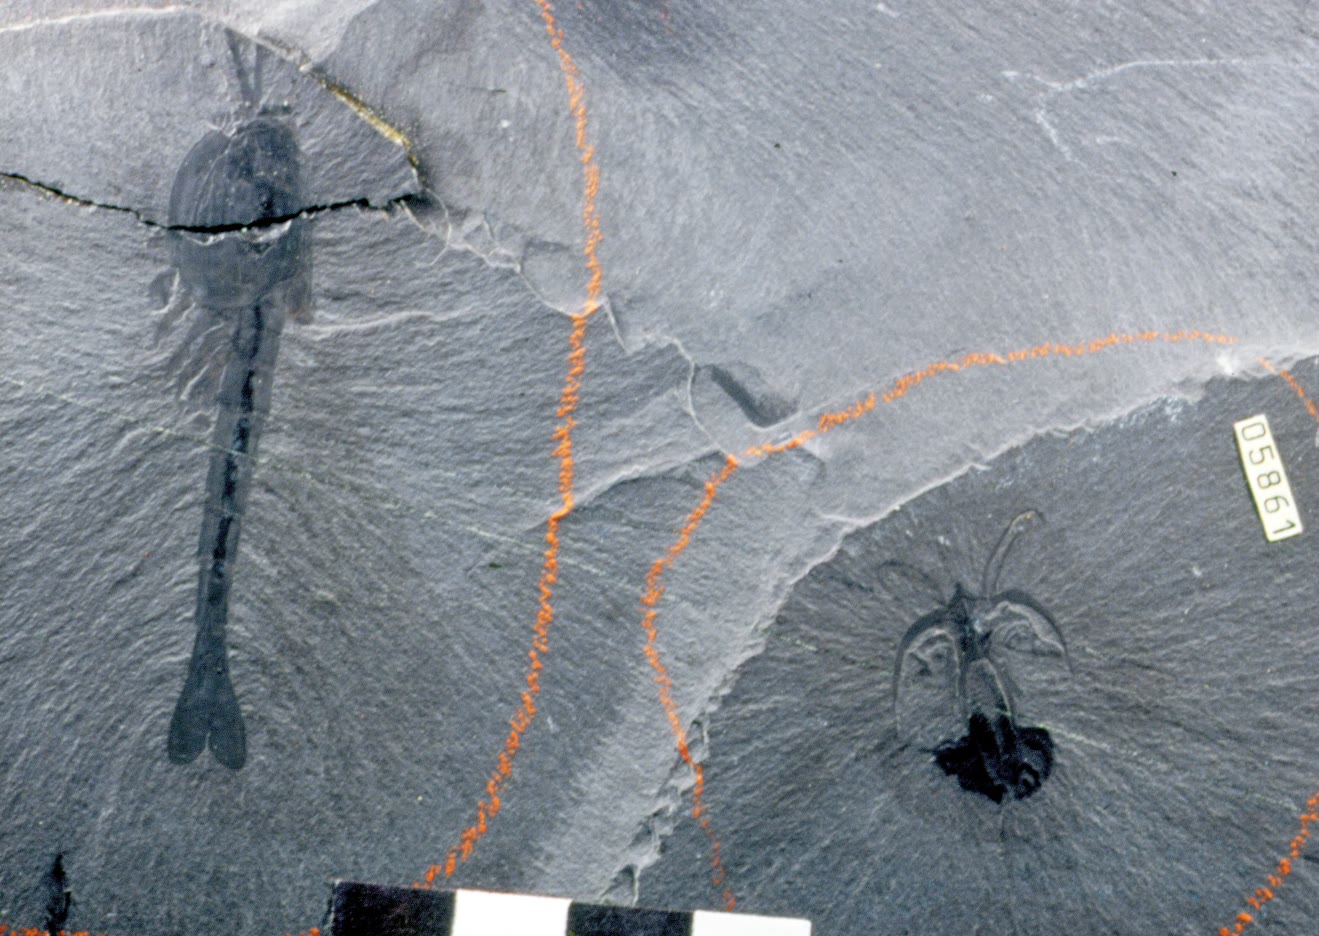
\includegraphics[width=0.72\linewidth]{images/book4/b2-20-burgess-waptia-marrella.jpg}
\par\smallskip{\small Dua artropoda dari Serpih Burgess, yang terawetkan sebagai lapisan tipis karbon yang gelap:
\emph{Waptia} (kiri) dan \emph{Marrella} (kanan).
(Foto: James St.~John, CC~BY~2.0, via Wikimedia Commons.)}
\end{omfigure}
% ledger: mussini25:burgess

\subsection*{Solnhofen}

Batu gamping berbutir halus di Solnhofen dan Eichstätt, di Bayern, diendapkan di laguna-laguna
pada awal Tithonium, kala terakhir Jura, yang dimulai \qty{149.2}{Ma} yang lalu. Batu gamping itu adalah
lokalitas tipe dua belas spesimen \emph{Archaeopteryx}, banyak pterosaurus, dan ikan
yang jaringan lunaknya dan bahkan pola warnanya masih terawetkan. Fosil di sana langka, tetapi
pengawetannya luar biasa. Beberapa kondisi telah diajukan, yang mungkin bekerja bersama-sama:
air dasar yang sekitar tiga kali lebih asin daripada air laut atau sangat basa, yang memperlambat pembusukan
oleh bakteri; tikar bakteri yang menyegel bangkai-bangkai; air dasar tanpa oksigen, yang menjauhkan
pemakan bangkai; dan badai yang mengaduk lumpur gamping dan menimbun bangkai-bangkai dengan cepat. Masing-masing
kondisi itu memperpanjang waktu bertahan $1/k$ atau memperpendek waktu sampai tertimbun $h/s$.
% ledger: gerschermann21:solnhofen, rauhut18:archaeopteryx, ics4:jurassic-stages

\begin{omfigure}
\centering
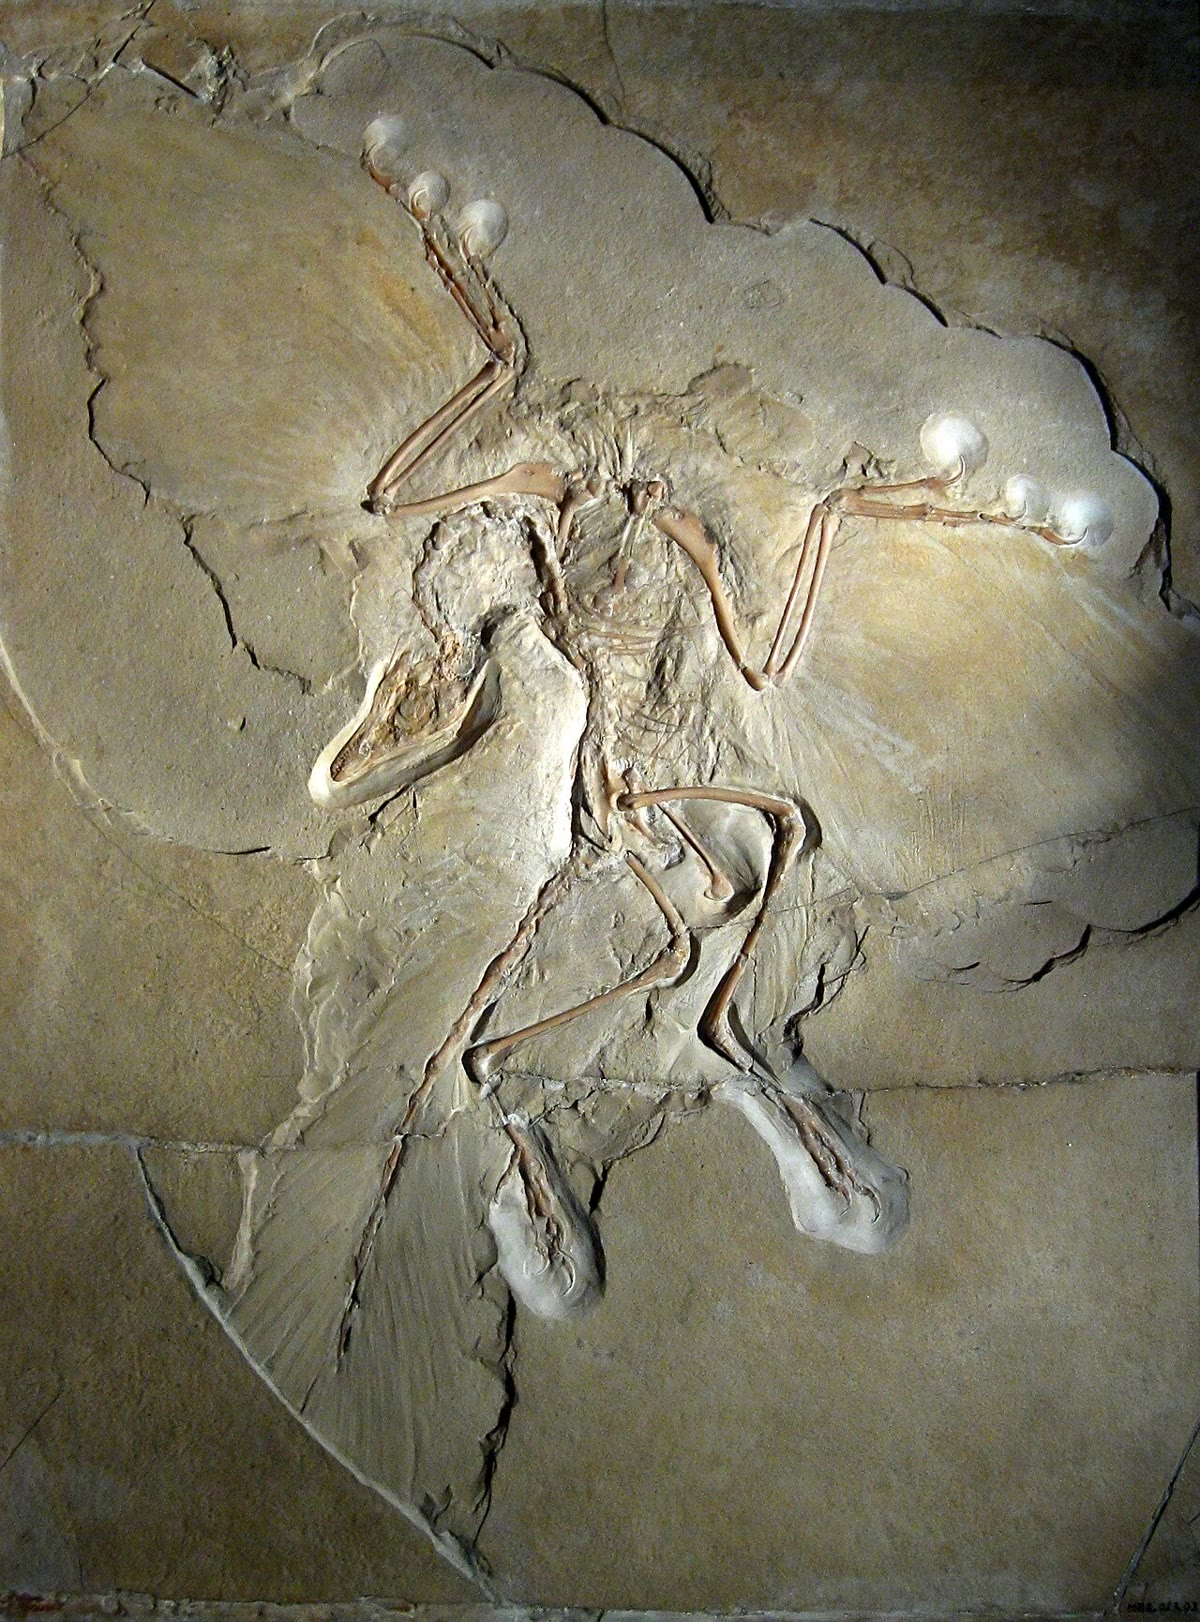
\includegraphics[width=0.5\linewidth]{images/book4/b2-20-archaeopteryx-berlin.jpg}
\par\smallskip{\small Spesimen Berlin \emph{Archaeopteryx}, dari batu gamping
Solnhofen: tulang-tulang dan jejak bulu sayap dan ekornya.
(Foto: H.~Raab, CC~BY-SA~3.0, via Wikimedia Commons.)}
\end{omfigure}
% ledger: rauhut18:archaeopteryx, gerschermann21:solnhofen

\subsection*{Fosil sebagai jam}

Volume Tahun 1 membangun biozona, yaitu satu tubuh strata yang ditentukan oleh fosilnya, dan fosil
indeks yang mengenalinya. Sehalus apa jam yang dihasilkannya? Sebuah zona amonit Jura dapat berlangsung
sekitar sejuta tahun: zona Toarsium yang paling awal, yang umurnya ditentukan dengan umur uranium--timbal lapisan abu di
Argentina, meliputi 183.73 sampai \qty{182.77}{Ma}. Zona dibagi menjadi horizon, dan pada Jura
Akhir sebuah horizon amonit rata-rata berlangsung \qty{165}{ka}. Semua kerangka
\emph{Archaeopteryx} berasal dari satu zona yang memuat lima horizon, sehingga burung itu dikenal selama
sekitar 0.7 sampai 1 juta tahun. Namun fosil hanya memberikan urutan; umur dalam tahun berasal
dari lapisan abu yang ditentukan umurnya dengan uranium dan timbal, dan dari siklus sedimen. Lapisan abu yang sama menempatkan alas Toarsium pada $183.73$, dengan ketidakpastian
$+0.35$ dan \qty{-0.50}{Ma}, sedangkan bagan internasional memberikan \qty{184.2}{Ma}.
% ledger: alsuwaidi22:toarcian, rauhut18:archaeopteryx, ics4:jurassic-stages

\section{Fosil sebagai saksi lingkungan}\label{sec:b2:palaeoenvironments:environment}

Untuk membaca suatu lingkungan dalam fosil, seorang ahli geologi mengandaikan bahwa organisme itu hidup di tempat kerabatnya yang
masih hidup kini tinggal, dan bahwa proses-proses yang bekerja pada sedimen kini bekerja dengan cara yang sama pada masa itu.

\begin{definition}[Aktualisme]\label{def:b2:palaeoenvironments:actualism}
Yang disebut \emph{aktualisme}\index{aktualisme} adalah metode menafsirkan rekaman geologi masa lampau melalui
proses-proses, dan hubungan antara organisme dan lingkungannya, yang dapat diamati kini.
\end{definition}

Pada 1830 Charles Lyell memberi volume pertama \emph{Principles of Geology}-nya anak judul ``suatu
upaya untuk menjelaskan perubahan-perubahan permukaan Bumi pada masa lampau dengan merujuk pada sebab-sebab yang kini
bekerja''. Metode itu memiliki batas. Banyak kelompok telah punah, dan cara hidupnya harus
disimpulkan dari bentuknya dan dari sedimen di sekitarnya; dan suatu lingkungan masa lampau mungkin
tidak memiliki padanan yang tepat pada masa kini.
% ledger: lyell1830:title

\begin{definition}[Paleolingkungan]\label{def:b2:palaeoenvironments:palaeoenvironment}
Yang disebut \emph{paleolingkungan}\index{paleolingkungan} adalah himpunan kondisi fisik, kimia, dan
biologi yang berlaku di tempat dan pada waktu suatu batuan terbentuk: tatanan, kedalaman dan
energi air, salinitasnya, suhunya, dan oksigennya, sifat dasarnya, serta kehidupan
di atasnya.
\end{definition}

\subsection*{Di mana fosil itu hidup?}

Pertanyaan pertama adalah apakah fosil-fosil itu hidup di tempat ia kini terbaring.

\begin{definition}[Kumpulan hidup dan kumpulan mati; fosil autokton dan alokton]\label{def:b2:palaeoenvironments:assemblages}
Yang disebut \emph{kumpulan hidup}\index{kumpulan hidup} adalah sekelompok fosil organisme yang hidup
bersama, terawetkan di tempat dan dalam keadaan saat organisme itu hidup; \emph{kumpulan mati}\index{kumpulan mati} adalah
sekelompok sisa yang terkumpul setelah kematian, yang dapat mencampurkan organisme dari tempat yang berbeda
dan waktu yang berbeda. Suatu fosil disebut \emph{autokton}\index{fosil autokton} jika ia
terawetkan di tempat organisme itu hidup, dan \emph{alokton}\index{fosil alokton} jika ia
diangkut dari tempat lain sebelum tertimbun.
\end{definition}

Petunjuknya adalah petunjuk pengangkutan. Cangkang yang masih tertutup, koral atau bivalvia penggali dalam
posisi tumbuhnya, duri-duri halus yang utuh, semua umur suatu populasi hadir: fosil-fosil itu
kemungkinan \omterm{def:b2:palaeoenvironments:assemblages}{autokton}. Katup-katup tunggal yang terpilah menurut ukuran, pecahan yang aus dan patah, cangkang yang
terkonsentrasi di alas lapisan bergradasi: semuanya telah terangkut. \omterm{def:b2:palaeoenvironments:assemblages}{Kumpulan mati} cangkang, seperti
kumpulan di dasar pesisir di atas, masih memuat sebagian besar komunitas, tetapi kumpulan itu menghimpun bertahun-tahun
komunitas itu ke dalam satu lapisan: fosil-fosilnya dirata-ratakan terhadap waktu.
% ledger: tyler25:live-dead

\subsection*{Salinitas dan oksigen}

Sebagian hewan hanya menoleransi salinitas laut terbuka: hewan itu disebut stenohalin. Ekinodermata,
sefalopoda, koral, dan, pada Paleozoikum, trilobit adalah kelompok stenohalin yang khas; kehadirannya
menunjukkan air laut yang normal, dan ketidakhadirannya dari suatu fauna yang kaya dapat menunjukkan sebaliknya.
Endapan sebuah estuari Silur di Vietnam memuat serpihan tumbuhan, tulang ikan, bivalvia, gastropoda,
dan ostrakoda, tetapi tidak satu pun dari kelompok-kelompok tadi. Ekinodermata juga tidak ada dalam biota Chengjiang,
sebuah \omterm{def:b2:palaeoenvironments:lagerstatte}{Lagerstätte} berumur sekitar 518 juta tahun, walaupun ekinodermata terdapat dalam Lagerstätten laut terbuka
Kambrium: hewan-hewan Chengjiang hidup di lepas sebuah delta, tempat air tawar membuat salinitas berfluktuasi.
% ledger: mcgairy21:stenohaline, saleh22:echinoderms, saleh22:age

Oksigen meninggalkan tandanya melalui para penggali liang. Di tempat air dasar mengandung oksigen, hewan-hewan mengaduk
sedimen dan menghancurkan laminasi halusnya; di tempat air itu tidak mengandung oksigen, laminanya bertahan, liang
tidak ada, dan pirit terbentuk, seperti dalam serpih hitam \omterm{def:b2:phanerozoic-earth:oae}{peristiwa anoksik samudra} pada
\cref{ch:b2:phanerozoic-earth}. Ketiadaan penggali liang yang sama melindungi bangkai-bangkai di Serpih
Burgess.
% ledger: mussini25:burgess

\subsection*{Iknofasies}

\omterm{def:b2:palaeoenvironments:fossil-kinds}{Fosil jejak} adalah saksi terbaik tentang dasar, karena \omterm{def:b2:palaeoenvironments:fossil-kinds}{fosil jejak} tidak berpindah. Pembuatnya
menanggapi energi air, kekerasan dasar, makanan, dan oksigen, dan
asosiasi jejak yang sama berulang sepanjang Fanerozoikum.

\begin{definition}[Iknofasies]\label{def:b2:palaeoenvironments:ichnofacies}
Yang disebut \emph{iknofasies}\index{iknofasies} adalah asosiasi \omterm{def:b2:palaeoenvironments:fossil-kinds}{fosil jejak} yang berulang dan yang
mencerminkan seperangkat kondisi lingkungan; iknofasies dinamai menurut sebuah jejak yang khas.
\end{definition}

Di sepanjang profil laut, dari pantai sampai cekungan dalam, empat \omterm{def:b2:palaeoenvironments:ichnofacies}{iknofasies} laut susul-menyusul
(gambar di bawah). \omterm{def:b2:palaeoenvironments:ichnofacies}{Iknofasies} \emph{Skolithos}, yang didominasi oleh liang hunian vertikal, berbentuk silinder atau
berbentuk U, milik pemakan suspensi, dengan sedikit jejak horizontal, khas untuk
pantai depan dan muka pantai. \omterm{def:b2:palaeoenvironments:ichnofacies}{Iknofasies} \emph{Cruziana}, yang didominasi oleh liang
pemakan endapan, dengan jejak perumput, karnivor, dan pemakan suspensi, khas untuk zona
lepas pantai: dasar antara dasar gelombang cuaca cerah, yaitu kedalaman yang di atasnya gelombang biasa mengaduk
sedimen, dan dasar gelombang saat badai, yang hanya dicapai oleh gelombang saat badai. \omterm{def:b2:palaeoenvironments:ichnofacies}{Iknofasies} \emph{Zoophycos},
yang dinamai menurut sebuah liang yang mengolah ulang sedimen dalam lembaran berpilin di sekeliling sumbu
pusat, khas untuk paparan di bawah dasar gelombang saat badai dan untuk lereng. \omterm{def:b2:palaeoenvironments:ichnofacies}{Iknofasies} \emph{Nereites},
dengan liang berkelok teratur, berbentuk spiral, dan berjaringan, yang dibaca sebagai perangkap dan
kebun hewan yang hanya menemukan sedikit makanan, khas untuk laut dalam di luar tepi paparan. Di
teluk payau dan estuari, \omterm{def:b2:palaeoenvironments:ichnofacies}{iknofasies} Cruziana dengan sedikit spesies adalah hal yang biasa.
% ledger: buatois20:ichnofacies, miguez21:ichnofacies, zhang15:zoophycos, buatois25:graphoglyptids, paz23:nereites

\begin{omfigure}
\centering
\begin{tikzpicture}[font=\scriptsize, x=1cm, y=1cm]
% sea and floor (schematic, not to scale)
\fill[omSea!20] (0.6,0) -- (14,0) -- (14,-3.6) -- (11.2,-3.6) -- (9.6,-1.9) -- (6.2,-1.5)
  -- (3.2,-0.9) -- (1.2,-0.15) -- cycle;
\fill[omLithSand!45] (0,0.25) -- (0.6,0) -- (1.2,-0.15) -- (3.2,-0.9) -- (6.2,-1.5)
  -- (9.6,-1.9) -- (11.2,-3.6) -- (14,-3.6) -- (14,-4.3) -- (0,-4.3) -- cycle;
\draw[black!70, line width=0.6pt] (0,0.25) -- (0.6,0) -- (1.2,-0.15) -- (3.2,-0.9) -- (6.2,-1.5)
  -- (9.6,-1.9) -- (11.2,-3.6) -- (14,-3.6);
\draw[omSea!80!black, line width=0.6pt] (0.6,0) -- (14,0);
\node[anchor=south east, omSea!80!black] at (14,0) {muka laut};
% wave bases
\draw[dashed, black!60] (2.133,-0.5) -- (14,-0.5) node[anchor=south east, black!70] {dasar gelombang cuaca cerah};
\draw[dashed, black!60] (4.7,-1.2) -- (14,-1.2) node[anchor=south east, black!70] {dasar gelombang saat badai};
% zone labels
\node[align=center] at (1.9,0.55) {pantai depan,\\muka pantai};
\node[align=center] at (4.6,0.55) {lepas pantai};
\node[align=center] at (8.0,0.55) {paparan};
\node[align=center] at (10.5,0.55) {lereng};
\node[align=center] at (12.7,0.55) {cekungan};
% Skolithos: vertical tubes
\foreach \x in {1.75,1.95,2.15,2.35} {\draw[black!80, line width=0.7pt] (\x,{-0.15-0.375*(\x-1.2)}) -- ++(0,-0.55);}
\node[align=center] at (2.1,-2.15) {\textbf{\emph{Skolithos}}\\tabung vertikal};
% Cruziana: horizontal bilobed trails
\foreach \x in {4.0,4.8} {\draw[black!80, line width=0.6pt] (\x,-1.45) .. controls ++(0.2,0.08) .. ++(0.5,0);
  \draw[black!80, line width=0.6pt] (\x,-1.53) .. controls ++(0.2,-0.08) .. ++(0.5,0);}
\node[align=center] at (4.7,-2.35) {\textbf{\emph{Cruziana}}\\liang makan,\\jejak merumput};
% Zoophycos: spreite arcs
\foreach \r in {0.12,0.22,0.32} {\draw[black!80, line width=0.5pt] (8.0,-2.25) ++(-\r,0) arc (180:360:\r cm and 0.5*\r cm);}
\draw[black!80, line width=0.6pt] (8.0,-2.25) -- (8.0,-1.8);
\node[align=center] at (8.0,-3.05) {\textbf{\emph{Zoophycos}}\\lembaran\\berpilin};
% Nereites: meander
\draw[black!80, line width=0.6pt, domain=0:2.2, samples=80, smooth] plot (12.0+\x*0.5,{-3.9+0.12*sin(\x*720)});
\node[align=center, anchor=north] at (12.5,-4.35) {\textbf{\emph{Nereites}}\\kelokan, jaringan};
\end{tikzpicture}
\par\smallskip{\small Keempat \omterm{def:b2:palaeoenvironments:ichnofacies}{iknofasies} laut dalam model Seilacher di sepanjang profil dari
pantai sampai cekungan dalam, dengan sketsa sebuah jejak yang khas untuk masing-masing; kedalamannya tidak menurut
skala. Jejak-jejak itu lebih menanggapi energi, makanan, dan oksigen daripada kedalaman itu sendiri.}
\end{omfigure}
% ledger: buatois20:ichnofacies, miguez21:ichnofacies, zhang15:zoophycos, buatois25:graphoglyptids, paz23:nereites

Kedalaman tidak bekerja secara langsung. Di sebuah saluran laut dalam, tempat arus turbidit kuat, liang
vertikal \omterm{def:b2:palaeoenvironments:ichnofacies}{iknofasies} Skolithos muncul jauh di bawah dasar gelombang mana pun; dan dekat sebuah delta, tempat air tawar
dan lumpur tercurah masuk, jejak lepas pantai lebih miskin daripada di tempat lain. Para pembuatnya juga berpindah
sepanjang waktu: liang \emph{Zoophycos} hidup di paparan pada Paleozoikum, di paparan bawah
dan lereng pada Mesozoikum, dan di laut dalam pada Kenozoikum. \omterm{def:b2:palaeoenvironments:ichnofacies}{Iknofasies} merekam
kondisi di dasar, sedangkan kedalaman hanya disimpulkan darinya, dan penyimpulan itu harus memakai
umur batuan.
% ledger: buatois20:ichnofacies, zhang15:zoophycos

\begin{inthefield}[Menghitung fosil lapis demi lapis]
Seorang ahli paleontologi yang merekonstruksi suatu lingkungan dari sebuah penampang mencatat setiap lapisan dengan
litologinya, ketebalannya, dan struktur sedimennya, lalu fosilnya: kelompok mana, berapa banyak,
apakah cangkangnya utuh atau patah, tertutup atau terbuka, terpilah atau tidak, dan dalam posisi apa cangkang itu terbaring.
\omterm{def:b2:palaeoenvironments:fossil-kinds}{Fosil jejak} dicatat di tempat fosil itu terlihat, pada bidang perlapisan dan pada muka vertikal,
dengan kedalaman yang dicapai liang. Karena cangkang dapat dipindahkan tetapi liang tidak, kedua
daftar itu dipisahkan; lingkungan dibaca terlebih dahulu dari jejak, dan \omterm{def:b2:palaeoenvironments:fossil-kinds}{fosil tubuh}
lalu diperiksa untuk mencari tanda-tanda pengangkutan.
\end{inthefield}

\begin{omfigure}
\centering
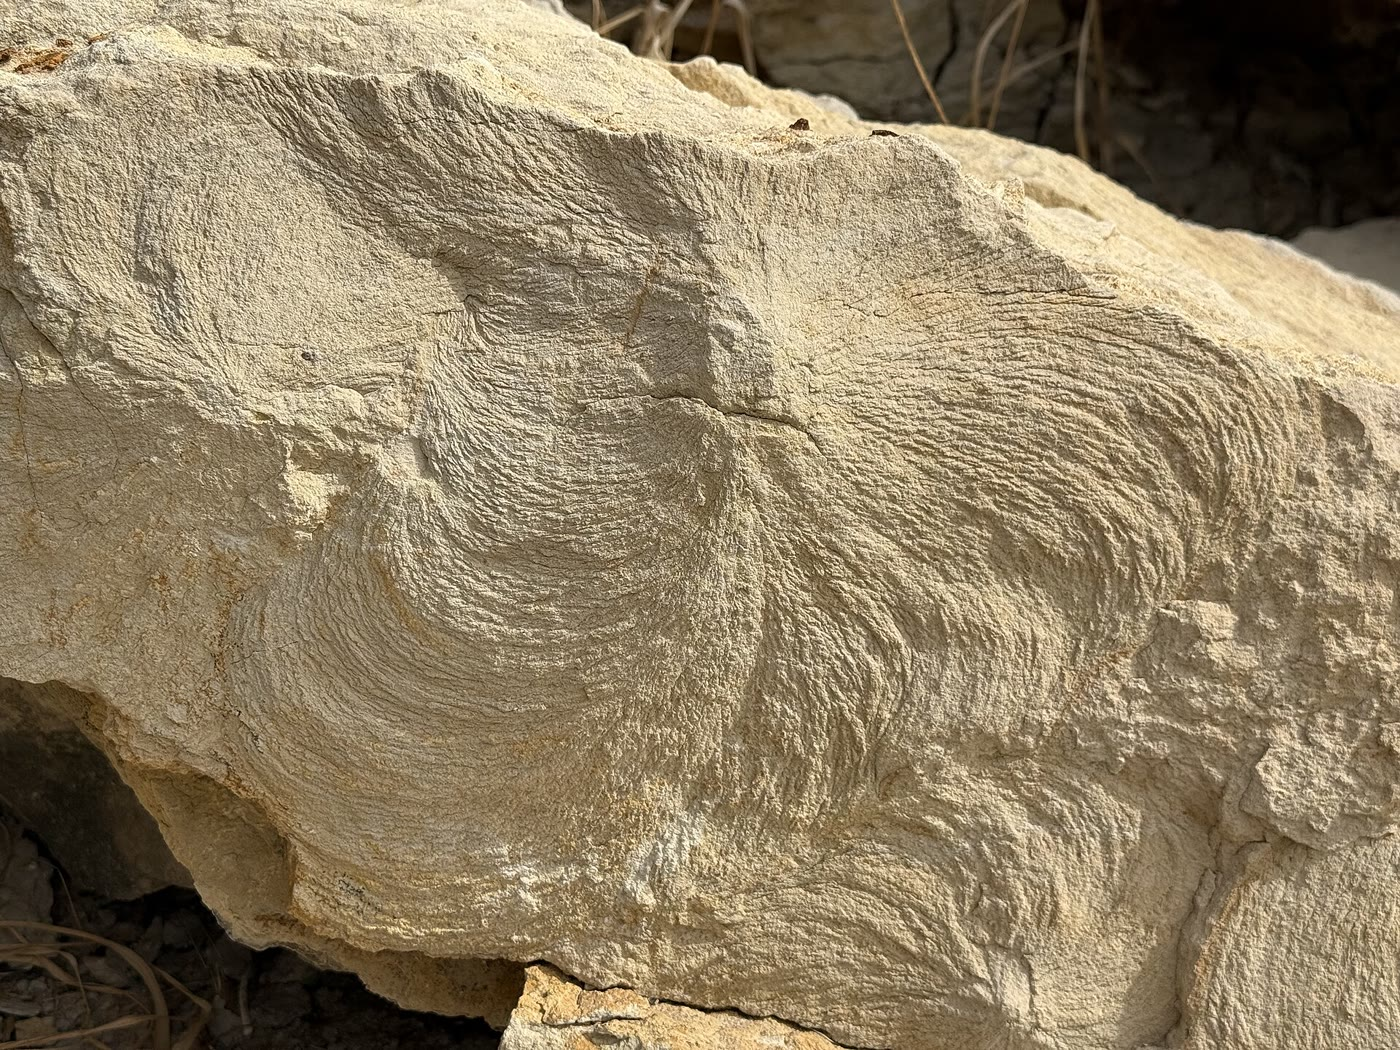
\includegraphics[width=0.5\linewidth]{images/book4/b2-20-zoophycos.jpg}
\par\smallskip{\small \emph{Zoophycos} dalam sebuah bongkah di Sagres, Portugal: busur-busurnya adalah lamela
sebuah lembaran berpilin dari sedimen yang diolah ulang. (Foto: Amada44, CC~BY~4.0, via Wikimedia Commons.)}
\end{omfigure}
% ledger: zhang15:zoophycos

\section{Membaca laut yang telah lenyap}\label{sec:b2:palaeoenvironments:varden}

Lingkungan-lingkungan terletak berdampingan: pantai, dasar lepas pantai, paparan yang lebih dalam. Ketika laut naik atau
dasar turun, setiap lingkungan bergerak ke arah daratan di atas tetangganya, dan endapannya menjadi terletak
di atas endapan tetangga itu. Dengan demikian suksesi vertikal fasies, tanpa jeda, mengulang
urutan lingkungan yang dulu terletak bersebelahan; volume Tahun 3 menjadikan aturan ini,
hukum Walther, titik tolaknya. Log yang dibaca dari bawah ke atas adalah sebuah film tentang pantai yang bergerak
melintasi satu tempat.

Penutup sedimen Perbukitan Varden, wilayah rekaan seri ini, memberikan contoh yang lengkap. Ketebalannya
adalah ketebalan dalam model wilayah itu; fosil-fosil pada gambar di bawah direka untuknya,
tetapi masing-masing dipilih sebagai fosil yang dapat dimuat oleh batuan nyata sejenis. Batu gamping diberi umur
Toarsium, dari 184.2 sampai \qty{174.7}{Ma}, dan serpih umur Aalenium sampai Callovium, dari
\qty{174.7}{Ma} sampai \qty{161.5}{Ma}.
% ledger: data:b4-palaeoenv, ics4:jurassic-stages

\begin{omfigure}
\centering
% figdata/bachelor-2/palaeoenv.py part log (thicknesses from figdata/shared/region.py)
\begin{tikzpicture}[x=1cm, y=0.0165cm, font=\scriptsize]
% scale
\draw[black!70] (-0.35,0) -- (-0.35,460);
\foreach \z in {0,100,...,400} {\draw[black!70] (-0.45,\z) -- (-0.35,\z) node[left=3pt] {\z};}
\node[rotate=90, anchor=south] at (-1.15,230) {tinggi di atas alas penutup sedimen (m)};
% units
\fill[lith sandstone] (0,0) rectangle (2.2,120);
\fill[lith limestone] (0,120) rectangle (2.0,180);
\fill[lith limestone] (0,180) rectangle (1.6,300);
\fill[lith shale] (0,300) rectangle (1.1,400);
\fill[om lith={icsCretaceous!35}{om limestone}] (0,400) -- (1.4,400) -- (1.4,452)
  .. controls (1.0,466) and (0.6,446) .. (0.3,458) -- (0,455) -- cycle;
\draw[black!70] (0,0) rectangle (2.2,120);
\draw[black!70] (0,120) rectangle (2.0,180);
\draw[black!70] (0,180) rectangle (1.6,300);
\draw[black!70] (0,300) rectangle (1.1,400);
\draw[black!70] (0,400) -- (1.4,400) -- (1.4,452) .. controls (1.0,466) and (0.6,446) ..
  (0.3,458) -- (0,455) -- cycle;
\node[anchor=west, font=\tiny] at (1.45,460) {puncak tererosi};
% unit names
\node[anchor=west, align=left] at (2.6,60) {\textbf{batu pasir}\\\qty{120}{m}, Trias};
\node[anchor=west, align=left] at (2.6,150) {\textbf{batu gamping oolitik}\\\qty{60}{m}, Toarsium};
\node[anchor=west, align=left] at (2.6,240) {\textbf{batu gamping halus}\\\qty{120}{m}, Toarsium};
\node[anchor=west, align=left] at (2.6,350) {\textbf{serpih}\\\qty{100}{m}, Aalenium--Callovium};
\node[anchor=west, align=left] at (2.6,424) {\textbf{kapur}\\Kapur};
% content
\node[anchor=west, align=left, text width=6.9cm] at (6.3,60) {isian saluran berperlapisan silang di atas alas
  tergerus; jejak akar; pecahan tumbuhan; tanpa fosil laut};
\node[anchor=west, align=left, text width=6.9cm] at (6.3,150) {ooid berperlapisan silang; tabung vertikal
  dan liang berbentuk U; pecahan cangkang yang aus};
\node[anchor=west, align=left, text width=6.9cm] at (6.3,240) {osikel krinoid, brakiopoda,
  belemnit, amonit; jejak merayap dan liang makan; lapisan cangkang patah dengan alas
  yang tajam};
\node[anchor=west, align=left, text width=6.9cm] at (6.3,350) {kelabu gelap, setempat berlaminasi;
  pirit; amonit dan bivalvia bercangkang tipis; liang spreite berpilin di lapisan yang lebih pucat};
\node[anchor=west, align=left, text width=6.9cm] at (6.3,424) {kokolit; ekinoid, spons;
  nodul rijang; terbioturbasi di seluruhnya};
\foreach \z in {120,180,300,400} {\draw[black!25] (2.25,\z) -- (13.2,\z);}
\node[font=\scriptsize\bfseries, anchor=south west] at (2.6,462) {satuan dan umur};
\node[font=\scriptsize\bfseries, anchor=south west] at (6.3,462) {apa yang dimuat lapisan};
\end{tikzpicture}
\par\smallskip{\small Penutup sedimen Perbukitan Varden sebagai log, dengan isi satuan-satuannya.
Ketebalannya adalah ketebalan dalam model wilayah itu, kecuali kapur, yang puncaknya tererosi dan dipotong di sini
(setebal \qty{766}{m} di sinklin pada \cref{ex:b2:palaeoenvironments:shale}); lebar kolom bertambah dengan ukuran butir;
fosil dan umurnya direka untuk wilayah itu.}
\end{omfigure}
% ledger: data:b4-palaeoenv, ics4:jurassic-stages

\begin{example}[Alas penutup sedimen Varden]\label{ex:b2:palaeoenvironments:base}
Batu pasir memuat isian saluran di atas alas tergerus, akar, dan pecahan tumbuhan, dan tidak memuat fosil
laut: batu pasir itu diendapkan oleh sungai di darat. Batu gamping oolitik di atasnya memiliki ooid berperlapisan silang,
yang tumbuh sambil berguling di air yang bergolak, tabung vertikal dan liang berbentuk U dari \omterm{def:b2:palaeoenvironments:ichnofacies}{iknofasies}
Skolithos, dan pecahan cangkang yang aus, semuanya \omterm{def:b2:palaeoenvironments:assemblages}{alokton}: sebuah gosong di muka pantai,
yang disapu gelombang. Di antara keduanya laut datang: kontak itu merekam suatu \omterm{def:b2:phanerozoic-earth:transgression}{transgresi laut}. Dalam
urutan hukum Walther, dataran sungai disusul oleh pantai, lalu oleh gosong.
\end{example}
% ledger: buatois20:ichnofacies

\subsection*{Seberapa cepat dasar laut terisi?}

Biozona memberikan durasi, log memberikan ketebalan, dan rasio keduanya adalah laju. Tetapi
ketebalan itu telah menyusut sejak sedimen diendapkan: air dalam pori telah terperas
keluar, dan hanya butirannya yang kekal.

\begin{proposition}[Laju akumulasi lapisan yang terkompaksi]\label{prop:b2:palaeoenvironments:rate}
Lapisan yang ketebalannya kini $h$ dan porositas rata-ratanya $\varphi$, yang diendapkan selama waktu $\Delta t$
dengan porositas $\varphi_0$, terakumulasi dengan laju
\[
  r = \frac{h\,(1 - \varphi)}{(1 - \varphi_0)\,\Delta t}
\]
sedimen segar, dan dengan laju $h(1-\varphi)/\Delta t$ butiran, yang tidak bergantung pada
$\varphi_0$.
\end{proposition}

\begin{proof}
Per satuan luas, lapisan itu memuat volume butiran $h(1 - \varphi)$, yaitu ketebalan padat pada
volume Tahun 1. Kompaksi mengusir air tetapi tidak menambah ataupun mengurangi butiran, sehingga sedimen
segar, dengan porositas $\varphi_0$, memiliki ketebalan $h_0$ dengan $h_0(1 - \varphi_0) = h(1 -
\varphi)$. Membagi $h_0$ dan ketebalan padat dengan $\Delta t$ memberikan kedua laju itu.
\end{proof}

Bila porositas tidak diukur, hukum Athy memberikannya dari kedalaman. Gambar di bawah menunjukkan
hukum itu untuk empat litologi, dan faktor $(1 - \varphi(z))/(1 - \varphi_0)$ yang dengannya lapisan
tipis yang kini berada pada kedalaman $z$ harus direntangkan untuk memberikan ketebalannya di permukaan. Kapur dan serpih
mula-mula mengandung banyak air dan cepat kehilangannya: lapisan tipis serpih pada \qty{1000}{m} dulu 1.68 kali
lebih tebal ketika diendapkan, dan lapisan kapur 2.19 kali.
% ledger: pybacktrack:compaction, pybacktrack4:limestone, data:b4-palaeoenv

\begin{omfigure}
\centering
% figdata/bachelor-2/palaeoenv.py parts poro and ratio
\begin{tikzpicture}
\begin{groupplot}[group style={group size=2 by 1, horizontal sep=1.6cm},
  width=0.46\linewidth, height=6.2cm, y dir=reverse, ymin=0, ymax=3000,
  tick label style={font=\scriptsize}, label style={font=\small}, xtick pos=bottom,
  ytick pos=left, scaled y ticks=false, yticklabel style={/pgf/number format/1000 sep={\,}}]
\nextgroupplot[xmin=0, xmax=0.75, xlabel={porositas $\varphi$}, ylabel={kedalaman $z$ (\unit{m})},
  legend style={at={(0.5,1.04)}, anchor=south, draw=none, font=\scriptsize, legend columns=2}]
\addplot[omThm, line width=1pt] table[x=shale, y=z_m] {figdata/out/bachelor-2-palaeoenv-poro.dat};
\addlegendentry{serpih}
\addplot[omSea!80!black, line width=1pt, dashed] table[x=sandstone, y=z_m] {figdata/out/bachelor-2-palaeoenv-poro.dat};
\addlegendentry{batu pasir}
\addplot[black, line width=1pt, dotted] table[x=chalk, y=z_m] {figdata/out/bachelor-2-palaeoenv-poro.dat};
\addlegendentry{kapur}
\addplot[green!45!black, line width=1pt, dash dot] table[x=limestone, y=z_m] {figdata/out/bachelor-2-palaeoenv-poro.dat};
\addlegendentry{batu gamping}
\nextgroupplot[xmin=1, xmax=3.2, xlabel={faktor pemulihan $(1-\varphi)/(1-\varphi_0)$}]
\addplot[omThm, line width=1pt] table[x=shale, y=z_m] {figdata/out/bachelor-2-palaeoenv-ratio.dat};
\addplot[omSea!80!black, line width=1pt, dashed] table[x=sandstone, y=z_m] {figdata/out/bachelor-2-palaeoenv-ratio.dat};
\addplot[black, line width=1pt, dotted] table[x=chalk, y=z_m] {figdata/out/bachelor-2-palaeoenv-ratio.dat};
\addplot[green!45!black, line width=1pt, dash dot] table[x=limestone, y=z_m] {figdata/out/bachelor-2-palaeoenv-ratio.dat};
\end{groupplot}
\end{tikzpicture}
\par\smallskip{\small Kiri: porositas terhadap kedalaman menurut hukum Athy, dengan konstanta Sclater
dan Christie (1980) untuk serpih, batu pasir, dan kapur, serta konstanta Turer dan Maynard (2003) untuk batu gamping,
sebagaimana ditabulasikan dalam pyBacktrack. Kanan: faktor yang dengannya lapisan tipis pada kedalaman $z$
dipulihkan ke ketebalannya di permukaan.}
\end{omfigure}
% ledger: pybacktrack:compaction, pybacktrack4:limestone, data:b4-palaeoenv

\begin{example}[Serpih Varden]\label{ex:b2:palaeoenvironments:shale}
Di sinklin Perbukitan Varden kapur setebal \qty{766}{m}, sehingga serpih terletak antara
766 dan \qty{866}{m}. Dengan konstanta serpih, $\varphi_0 = 0.63$ dan $\lambda =
\qty{1960}{m}$, ketebalan padat pada volume Tahun 1 adalah $100 - 0.63 \times 1960 \times
(e^{-766/1960} - e^{-866/1960}) = \qty{58.4}{m}$, yaitu porositas rata-rata 0.416. Jika dibawa kembali ke
permukaan dengan butiran yang sama, lapisan itu setebal \qty{148.6}{m}. Selama \qty{13.2}{Ma} dari
alas Aalenium sampai puncak Callovium, serpih terakumulasi dengan laju $100/13.2 =
\qty{7.6}{m}$ per juta tahun menurut ketebalannya kini, $148.6/13.2 = \qty{11.3}{m}$ per juta
tahun lumpur segar, dan \qty{4.4}{m} per juta tahun butiran. Ketebalan masa kini
mengecilkan laju itu sepertiganya.
\end{example}
% ledger: data:b4-palaeoenv, pybacktrack:compaction, ics4:jurassic-stages

Serpih itu mungkin dulu terletak lebih dalam lagi, di bawah kapur yang sejak itu tererosi; koreksi itu lalu merupakan
nilai minimum. Soal akhir pekan menerapkan proposisi itu pada batu gamping, yang porositasnya
diukur.

\section*{Latihan}\label{sec:b2:palaeoenvironments:exercises}

Data untuk latihan, kecuali dinyatakan lain: hukum Athy $\varphi = \varphi_0 e^{-z/\lambda}$
dengan $\varphi_0 = 0.63$, $\lambda = \qty{1960}{m}$ (serpih), $0.49$, \qty{3704}{m} (batu pasir),
$0.70$, \qty{1408}{m} (kapur), $0.51$, \qty{4545}{m} (batu gamping); kalsit \qty{2710}{kg.m^{-3}},
air pori \qty{1000}{kg.m^{-3}}; umur pada bagan internasional: Toarsium 184.2 sampai
\qty{174.7}{Ma}.
% ledger: pybacktrack:compaction, pybacktrack4:limestone, ics4:jurassic-stages

\begin{exercise}[$\star$]\label{exo:b2:palaeoenvironments:1}
Di 51 lokasi pada dasar pesisir, 135 spesies avertebrata ditemukan hidup, 150 di antara cangkang dan
kerangka mati di dasar, dan 112 yang juga memiliki catatan fosil. (a) Nyatakan bilangan
ketiga sebagai fraksi dari masing-masing dua bilangan pertama. (b) Bagaimana yang mati bisa lebih banyak daripada yang hidup? (c)
Kelompok makan mana yang kamu duga kurang terwakili di antara yang mati, dan mengapa?
\end{exercise}
% ledger: tyler25:live-dead, tyler25:soft-bodied

\begin{exercise}[$\star$]\label{exo:b2:palaeoenvironments:2}
Sebuah horizon amonit Jura Akhir rata-rata berlangsung \qty{165}{ka}. (a) Berapa lama lima horizon
berlangsung? Bandingkan dengan 0.7 sampai 1 juta tahun yang diberikan untuk \emph{Archaeopteryx}. (b) Zona Toarsium
yang paling awal meliputi 183.73 sampai \qty{182.77}{Ma}: berapa horizon dengan panjang rata-rata yang akan dimuatnya?
(c) Mengapa horizon, bukan zona, yang penting untuk mengikuti evolusi suatu garis keturunan?
\end{exercise}
% ledger: rauhut18:archaeopteryx, alsuwaidi22:toarcian

\begin{exercise}[$\star$]\label{exo:b2:palaeoenvironments:3}
Sebutkan \omterm{def:b2:palaeoenvironments:ichnofacies}{iknofasies} dan tatanan setiap kumpulan jejak. (a) Jejak merumput yang berkelok-kelok dan jaringan liang
yang teratur pada alas turbidit tipis. (b) Tabung vertikal yang rapat dalam pasir bersih
berperlapisan silang. (c) Liang horizontal pemakan endapan yang melimpah dan jejak merumput dalam lapisan
lanauan di antara pasir badai. (d) Liang spreite berpilin dalam lumpur halus yang gelap tanpa riak
gelombang, dalam batuan Mesozoikum.
\end{exercise}
% ledger: buatois20:ichnofacies, paz23:nereites

\begin{exercise}[$\star$]\label{exo:b2:palaeoenvironments:4}
Lapisan A memuat krinoid, brakiopoda, koral, dan trilobit; lapisan B, yang seumur, memuat serpihan
tumbuhan, tulang ikan, beberapa bivalvia dan gastropoda, dan banyak individu dari hanya dua spesies
ostrakoda. (a) Apa yang dikatakan masing-masing tentang salinitas airnya? (b) Lapisan B tidak memiliki kelompok-kelompok
lapisan A: mengapa ketiadaan itu merupakan argumen, sedangkan ketiadaan satu fosil dari satu lapisan bukan argumen?
(c) Pengamatan lain mana yang akan menguji tafsiran lapisan B?
\end{exercise}
% ledger: mcgairy21:stenohaline, saleh22:echinoderms

\begin{exercise}[$\star\star$]\label{exo:b2:palaeoenvironments:5}
Gunakan \cref{prop:b2:palaeoenvironments:burial} dengan cangkang pada
\cref{ex:b2:palaeoenvironments:shell}, $k = \qty{0.05}{yr^{-1}}$ dan $h = \qty{0.1}{m}$. (a)
Tentukan laju sedimentasi yang membuat separuh cangkang mencapai keadaan aman. (b) Dengan faktor berapa $P$
berubah bila laju itu dibagi dua dari nilai tersebut? (c) Cangkang yang dua kali lebih tebal bertahan dua kali lebih lama
di dasar. Pada \qty{1}{mm.yr^{-1}}, berapa kali lebih besar peluangnya untuk terawetkan? (d) Apa
implikasinya bagi proporsi cangkang tipis dan cangkang tebal dalam suatu kumpulan fosil?
\end{exercise}
% ledger: tyler25:soft-bodied

\begin{exercise}[$\star\star$]\label{exo:b2:palaeoenvironments:6}
Lapisan abu menempatkan alas Toarsium di Chacay Melehue pada $183.73$, $+0.35$, \qty{-0.50}{Ma};
bagan internasional memberikan \qty{184.2}{Ma}. (a) Apakah nilai bagan itu berada dalam ketidakpastian?
Seberapa jauh nilai itu meleset dari batas atas? (b) Zona Toarsium yang paling awal berakhir pada
\qty{182.77}{Ma}: tentukan durasinya. (c) Misalkan zona ini setebal \qty{6}{m} dalam sebuah penampang:
berapa laju akumulasinya? (d) Mengapa suatu biozona dapat sama waktunya di mana-mana sementara
ketebalannya berbeda dari satu tempat ke tempat lain?
\end{exercise}
% ledger: alsuwaidi22:toarcian, ics4:jurassic-stages

\begin{exercise}[$\star\star$]\label{exo:b2:palaeoenvironments:7}
Di sinklin Varden batu pasir terletak antara 1046 dan \qty{1166}{m} di bawah permukaan tanah. (a)
Tentukan porositasnya menurut hukum Athy di puncak dan di alasnya, dan porositas rata-ratanya, dibulatkan sampai
tiga desimal, dari rata-rata keduanya. (b) Tentukan ketebalan padatnya. (c) Pulihkan lapisan itu ke
permukaan dengan faktor lapisan tipis pada porositas rata-rata. (d) Pemulihan yang eksak memberikan
\qty{147.0}{m}. Mengapa perkiraan lapisan tipis sedikit terlalu besar?
\end{exercise}
% ledger: data:b4-palaeoenv, pybacktrack:compaction

\begin{exercise}[$\star\star$]\label{exo:b2:palaeoenvironments:8}
Log densitas membaca \qty{2573}{kg.m^{-3}} pada batu gamping Varden, yang tersusun atas butiran kalsit dengan
air dalam pori-porinya. (a) Tunjukkan bahwa porositasnya $\varphi = (\rho_{\text{butir}} -
\rho)/(\rho_{\text{butir}} - \rho_{\text{air}})$ dan hitunglah. (b) Pada kedalaman tengah
batu gamping di sinklin, \qty{956}{m}, berapa yang diramalkan hukum Athy dengan konstanta batu gamping?
(c) Proses diagenesis mana yang dapat menjelaskan selisihnya?
\end{exercise}
% ledger: pybacktrack4:limestone, data:b4-palaeoenv

\begin{exercise}[$\star\star$]\label{exo:b2:palaeoenvironments:9}
Sebuah tebing batuan Jura menunjukkan dari alas ke atas: turbidit tipis dengan kelokan teratur dan jaringan
liang; lumpur gelap dengan liang spreite berpilin; lapisan lanauan dengan liang pemakan endapan di antara
pasir badai; pasir bersih berperlapisan silang dengan
tabung vertikal; lalu batu bara dengan akar. (a) Tafsirkan setiap bagian. (b) Apakah air makin dalam atau
makin dangkal? (c) Sebutkan dua penyebab yang dapat menghasilkan suksesi ini, dan katakan apa yang akan memutuskan
di antara keduanya. (d) Mengapa lompatan tajam dari bagian pertama ke bagian keempat, tanpa bagian-bagian lainnya, merupakan
peringatan?
\end{exercise}
% ledger: buatois20:ichnofacies, paz23:nereites

\begin{exercise}[$\star\star\star$]\label{exo:b2:palaeoenvironments:10}
Seekor hewan bertubuh lunak bertahan di dasar rata-rata selama setahun ($k = \qty{1}{yr^{-1}}$), sebuah
cangkang selama seabad; keduanya aman di bawah $h = \qty{0.1}{m}$. (a) Bandingkan peluang
keduanya untuk terawetkan pada 1, 10, dan \qty{100}{mm.yr^{-1}}. (b) Tentukan laju yang membuat satu tubuh lunak dalam
seratus terawetkan. (c) Apakah laju seperti itu masuk akal selama berbulan-bulan? Jenis endapan apa yang menimbun
dasar lebih cepat? (d) Asumsi mana dari \cref{prop:b2:palaeoenvironments:burial} yang gagal untuk
endapan seperti itu, dan bagaimana perilaku rumus itu ketika asumsi itu gagal?
\end{exercise}

\begin{exercise}[$\star\star\star$]\label{exo:b2:palaeoenvironments:11}
(a) Tunjukkan bahwa faktor lapisan tipis $(1 - \varphi(z))/(1 - \varphi_0)$ diturunkan dari
\cref{prop:b2:palaeoenvironments:rate}. (b) Terapkan faktor itu pada kedalaman tengah serpih Varden,
\qty{816}{m}, untuk memulihkan serpih setebal \qty{100}{m}. (c) Bandingkan dengan \qty{148.6}{m} yang eksak pada
\cref{ex:b2:palaeoenvironments:shale}, dan jelaskan tanda selisihnya. (d) Tunjukkan bahwa
laju butiran, tidak seperti laju sedimen segar, dapat dibandingkan antara serpih dan batu gamping
tanpa mengetahui seberapa berpori masing-masing ketika diendapkan.
\end{exercise}
% ledger: data:b4-palaeoenv, pybacktrack:compaction

\begin{exercise}[$\star\star\star$]\label{exo:b2:palaeoenvironments:12}
Misalkan horizon amonit Toarsium rata-rata berlangsung \qty{165}{ka}, seperti horizon Jura Akhir.
(a) Berapa horizon yang akan dimuat oleh batu gamping Varden setebal \qty{180}{m}? (b) Ketebalan
batu gamping berapa yang diwakili oleh satu horizon kini, dan ketebalan sedimen segar berapa, mengingat
lapisan itu setebal \qty{338}{m} ketika diendapkan? (c) Agar yakin menemukan setiap horizon, seorang
ahli geologi mengambil sampel dengan jarak tidak lebih dari separuh ketebalan masa kini itu: berapa jarak itu, dan berapa banyak
sampel? (d) Mengapa beberapa horizon mungkin tetap tidak ditemukan?
\end{exercise}
% ledger: rauhut18:archaeopteryx, ics4:jurassic-stages, data:b4-palaeoenv

\begin{problem}[{Soal akhir pekan --- Laut Jura di Perbukitan Varden}]\label{pb:b2:palaeoenvironments:1}
Soal ini membaca lingkungan dan sejarah penutup sedimen Varden, dengan log pada
\cref{sec:b2:palaeoenvironments:varden} dan data latihan. Penutup sedimen itu miring
\ang{12} pada sayap-sayap lipatan; di sinklin, penutup itu ditembus oleh sebuah sumur.

\medskip\noindent\textbf{Bagian I --- Batuan dan ketebalannya.}
\begin{enumerate}
  \item Di tanah datar pada sebuah sayap, batu gamping tersingkap selebar \qty{866}{m}, diukur
        tegak lurus jurus. Tentukan ketebalan sebenarnya.
  \item Serpih tersingkap selebar \qty{481}{m}. Tentukan ketebalannya.
  \item Satuan mana yang tertua, dan berdasarkan prinsip apa?
  \item Di sumur, serpih mulai pada \qty{766}{m}, batu gamping pada \qty{866}{m}, dan
        batu pasir pada \qty{1046}{m} di bawah permukaan tanah. Periksalah ketebalan-ketebalannya.
  \item Kapur terpotong oleh permukaan tanah. Apa yang dapat dikatakan tentang ketebalannya ketika
        laut Kapur surut?
  \item Tentukan porositas kapur di permukaan dan di alas kapur di sumur.
\end{enumerate}

\medskip\noindent\textbf{Bagian II --- Lingkungan.}
\begin{enumerate}[resume]
  \item Apa yang dikatakan krinoid, brakiopoda, belemnit, dan amonit dalam batu gamping halus
        tentang airnya?
  \item \omterm{def:b2:palaeoenvironments:ichnofacies}{Iknofasies} mana yang dibentuk oleh jejak-jejaknya, dan di bagian profil yang mana?
  \item Apa yang direkam oleh lapisan cangkang patahnya yang beralas tajam?
  \item Serpih itu gelap, setempat berlaminasi, dengan pirit dan sedikit liang. Apa yang dikatakan hal itu
        tentang air dasarnya?
  \item Lapisan-lapisannya yang lebih pucat memuat liang spreite berpilin. \omterm{def:b2:palaeoenvironments:ichnofacies}{Iknofasies} mana, dan tatanan mana?
  \item Apakah amonit dalam serpih merupakan bagian dari \omterm{def:b2:palaeoenvironments:assemblages}{kumpulan hidup} di dasar? Jelaskan.
\end{enumerate}

\medskip\noindent\textbf{Bagian III --- Waktu dan laju.} Lapisan batu gamping terbawah memuat
amonit zona Toarsium pertama, lapisan teratas memuat amonit zona terakhir, dan serpih dimulai dengan
zona Aalenium pertama.
\begin{enumerate}[resume]
  \item Berapa lama batu gamping itu terakumulasi?
  \item Dengan laju berapa, menurut ketebalan batu gamping kini?
  \item Log densitas sumur membaca \qty{2573}{kg.m^{-3}} pada batu gamping. Tentukan
        porositasnya.
  \item Lumpur gamping diendapkan dengan porositas 0.51. Tentukan ketebalan sedimen segarnya.
  \item Tentukan laju sedimen segar.
  \item Tentukan laju butiran.
  \item Bandingkan dengan serpih pada \cref{ex:b2:palaeoenvironments:shale}. Apa yang ditunjukkan oleh perubahan
        laju itu tentang pasokan karbonat?
\end{enumerate}

\medskip\noindent\textbf{Bagian IV --- Laut di atas Varden.}
\begin{enumerate}[resume]
  \item Bacalah kolom dari batu pasir sampai kapur. Apakah laut maju atau mundur?
  \item Pada kurva jangka panjang Haq dan kawan-kawan, muka laut global berada sekitar 41, 57, dan
        \qty{86}{m} di atas muka laut kini pada 184, 174, dan \qty{162}{Ma}. Berapa besar kenaikannya selama
        pengendapan batu gamping, selama pengendapan serpih, dan seluruhnya?
  \item Misalkan dasar berubah dari kedalaman air \qty{5}{m} di gosong menjadi \qty{60}{m} di puncak
        serpih. Tentukan akomodasi yang tercipta dari alas batu gamping sampai puncak
        serpih, dengan menghitung ketebalan segar kedua satuan, dan laju rata-ratanya.
  \item Bagian mana darinya yang dapat dijelaskan oleh kenaikan global? Apa yang membuat sisanya?
  \item Sebagai ringkasan: dengan laju berapa lumpur gamping batu gamping Varden terakumulasi ketika
        diendapkan?
\end{enumerate}
\end{problem}
% ledger: data:b4-palaeoenv, ics4:jurassic-stages, pybacktrack4:limestone, pybacktrack:compaction, data:b4-sealevel, haq87:charts, buatois20:ichnofacies, mcgairy21:stenohaline
